%% sections/results.tex — Steps B6–B9 + tables
\section{Results}
\label{sec:results}

%% ═══════════════════════════════════════════════════════════════════════════
%% B6 — Multimodal vs Single-Modality Baselines
%% ═══════════════════════════════════════════════════════════════════════════

\subsection{Multimodal Fusion Outperforms Single-Modality Baselines}
\label{sec:baselines}

Within the DyAM framework, models restricted to a single data source
achieved repeated-seed (5~seeds~$\times$~10-fold) AUC values of
$0.616 \pm 0.001$ (TMB), $0.635 \pm 0.021$ (pathology IHC),
$0.673 \pm 0.020$ (CT radiomics), $0.676 \pm 0.013$ (genomics), and
$0.720 \pm 0.012$ (PD-L1~TPS) on the discovery cohort.
PD-L1~TPS was the strongest individual predictor, consistent with its role
as the biomarker in routine clinical use.

Fusing four data sources (CT radiomics, pathology IHC-G, genomics, and
PD-L1~TPS) under the same protocol raised the AUC to $0.760 \pm 0.022$,
exceeding the best single source by $0.040$~AUC; adding NLP-encoded clinical
variables raised it further to $0.783 \pm 0.016$
(Section~\ref{sec:nlp_auc}).
Evaluated on the single cross-validation partition used for the DeLong
confidence intervals reported in Tables~\ref{tab:auc_ihca} and
\ref{tab:auc_ihcg}, the same four-source configuration reached
AUC~$= 0.784$ [95\%~CI: 0.717--0.850] (IHC-G arm;
Table~\ref{tab:auc_ihcg}).
Multimodal fusion is therefore the primary driver of predictive performance
in this cohort, with no individual source approaching the discrimination of
the fused model.

%% ═══════════════════════════════════════════════════════════════════════════
%% B7 — OvO Attention Comparison
%% ═══════════════════════════════════════════════════════════════════════════

\subsection{OvO Competitive Attention Achieves Performance Comparable to Cooperative Attention with a Simpler Parameterization}
\label{sec:ovo}

In an initial exploratory screen across 20 modality configurations
evaluated with a single 10-fold cross-validation partition, the OvO
attention variant outperformed the original cooperative attention
in 7 of 20 cases (35\%), while the original model was superior in 9 of 20
cases (45\%), with 4 identical results (single-modality, where OvO reduces
to the original).
The mean AUC difference was $-0.32\%$ in favour of the original model overall.
The largest single-partition gains for OvO were observed for PDL1+Gen
($\Delta\text{AUC} = +3.27\%$, AUC 0.716 vs.\ 0.693) and Rad+Gen
($\Delta\text{AUC} = +2.23\%$; Table~\ref{tab:ovo}), while the largest
deficits occurred for configurations combining three or more modalities,
particularly when IHC-G or clinical labs were included
(largest deficit: Rad+IHC-A+Gen, $\Delta\text{AUC} = -4.94\%$).

Because a single CV partition can favour either model by chance, we
repeated this comparison as a confirmatory analysis using 5 independent
random partitions (5~seeds~$\times$~10-fold, patient labels re-shuffled per
seed) across the same 21 modality combinations used in the primary
paper-matched configuration set (Section~\ref{sec:baselines}), with paired
bootstrap significance testing on the resulting patient-level scores.
At the primary benchmark configuration (Rad+IHC-G+Gen+PDL1), OvO reached a
repeated-seed mean AUC of $0.773 \pm 0.020$ versus $0.760 \pm 0.022$ for the
original cooperative model ($\Delta\text{AUC} = +0.009$, 95\% bootstrap CI
$[-0.008, 0.027]$, $p = 0.313$); across all four primary benchmarks the two
models differed by at most $0.011$~AUC ($p \geq 0.17$).
Extending the comparison to all 21 modality combinations
(Table~\ref{tab:ovo_all21}), OvO's repeated-seed mean AUC exceeded the
original model's in 12 of 21 configurations and was lower in 5 of 21, with 4
identical (single-modality, where the two formulations coincide
algebraically).
This advantage was concentrated in the many-source regime: for
configurations fusing $k \geq 5$ input sources, OvO matched or exceeded
cooperative attention in 7 of 8 cases (mean $\Delta\text{AUC} = +0.009$,
range $-0.001$ to $+0.018$), whereas for $k = 2$--$4$ it led in only 5 of 9
cases with a far wider spread (mean $+0.003$, range $-0.028$ to $+0.045$).
Notably, this is the opposite of the pattern suggested by the
single-partition screen, which had favoured OvO at low modality counts;
the repeated-seed evaluation instead places OvO's small but consistent edge
in precisely the multi-source configurations the fusion model is intended
for.
These per-$k$ counts are descriptive: formal significance testing was
performed only at the four primary benchmarks, and the effect sizes involved
($\leq 0.018$~AUC) remain below the seed-to-seed standard deviation
($\approx 0.02$), so the trend should be read as a consistency pattern
rather than a demonstrated superiority.
The single-partition ``best-performing configuration'' identified in the
initial screen (OvO Rad+IHC-G+Gen+PDL1, AUC~$=0.8003$ [95\%~CI:
0.739--0.862]) illustrates how favourable a single partition can be: the
same configuration's repeated-seed mean AUC was $0.773$, and OvO's rank
relative to the cooperative model reversed once averaged across seeds.

As a further robustness check, we combined OvO attention with the
NLP-clinical encoding described in Section~\ref{sec:nlp_auc}, repeating the
same 21-combination, 5-seed evaluation with clinical text embeddings added
to each configuration.
OvO+NLP reproduced the same fusion-dependent improvement pattern observed
in the primary NLP-clinical analysis (Section~\ref{sec:nlp_auc}): AUC
improved relative to the no-clinical baseline in 15 of 21 configurations
(an identical set of configurations), and declined in the same six single-
or near-single-modality configurations where any clinical addition diluted
a strong standalone signal (PD-L1, radiomics-only, and similar).
At the primary benchmark, OvO+NLP reached a repeated-seed mean
AUC~$=0.782 \pm 0.017$, matching the $0.783 \pm 0.016$ obtained by the
repeated-seed NLP-clinical confirmation at the same configuration
(Section~\ref{sec:nlp_auc}).
Under the single-partition protocol, OvO+NLP reached AUC~$=0.8133$ at the
Rad+IHC-A+Gen+TMB+PDL1 configuration, the highest value obtained under
either evaluation protocol in this study.
This shows that OvO's simpler, $N$-parameter formulation (independent
per-modality scores compared against the mean of the others) delivers the
same NLP-clinical benefit as the cooperative model without the
$N \times N$ weight matrix, and that the clinical-encoding intervention,
not the choice of attention mechanism, is the source of that gain.
Table~\ref{tab:ovo} summarises the exploratory single-partition screen and
Table~\ref{tab:ovo_all21} gives the repeated-seed AUC of all three models
across all 21 configurations; the corresponding single-partition values are
provided in Supplementary Table~S3.


\begin{table}[H]
\caption{Top configurations from the exploratory, single-partition screen
  comparing OvO competitive attention and original cooperative attention.
  $\Delta$AUC is computed as OvO minus Original.
  Bold denotes the higher AUC for each row.
  As described in the text, these single-partition differences were not
  reproducible under repeated-seed evaluation (Table~\ref{tab:ovo_all21})
  and should be interpreted as an initial screen rather than a confirmed
  effect.
  Gen, genomics; Rad, CT radiomics; IHC-A/G, immunohistochemistry variants;
  PDL1, PD-L1 TPS score.}
\label{tab:ovo}
\begin{minipage}[t]{0.48\textwidth}
\centering
\footnotesize
\textit{OvO better ($\Delta > 0$)}\\[3pt]
\begin{tabular}{@{}p{2.5cm}ccc@{}}
\toprule
Configuration & Orig. & OvO & $\Delta$ \\
\midrule
PDL1+Gen           & 0.693 & \textbf{0.716} & +3.27\% \\
Rad+Gen            & 0.738 & \textbf{0.755} & +2.23\% \\
Rad+IHC-G+Gen+PDL1 & 0.784 & \textbf{0.800} & +2.10\% \\
Rad+IHC-A+Gen+PDL1 & 0.764 & \textbf{0.777} & +1.63\% \\
TMB+PDL1           & 0.705 & \textbf{0.715} & +1.42\% \\
\bottomrule
\end{tabular}
\end{minipage}
\hfill
\begin{minipage}[t]{0.48\textwidth}
\centering
\footnotesize
\textit{Original better ($\Delta < 0$)}\\[3pt]
\begin{tabular}{@{}p{2.5cm}ccc@{}}
\toprule
Configuration & Orig. & OvO & $\Delta$ \\
\midrule
Rad+IHC-A+Gen      & \textbf{0.757} & 0.719 & $-4.94\%$ \\
IHC-G+Gen          & \textbf{0.756} & 0.723 & $-4.33\%$ \\
Rad+IHC-A+Gen+PDL1+Labs & \textbf{0.768} & 0.747 & $-2.83\%$ \\
Rad+IHC-G+Gen      & \textbf{0.787} & 0.766 & $-2.66\%$ \\
Rad+IHC-G+Gen+PDL1+Labs & \textbf{0.788} & 0.783 & $-0.56\%$ \\
\bottomrule
\end{tabular}
\end{minipage}
\end{table}

\begin{table}[H]
\centering
\caption{Repeated-seed (5~seeds~$\times$~10-fold) AUC across all 21
  paper-matched modality combinations, for the original cooperative
  attention (DyAM), OvO competitive attention, and OvO combined with
  NLP-clinical encoding. $k$ is the number of fused input sources
  (CT radiomics contributes one source per lesion site).
  Bold marks the highest value in each row. For $k = 1$ OvO reduces
  algebraically to the cooperative formulation, hence the identical values.
  Configurations 8, 11, 18 and 21 are the primary benchmarks BM4, BM3, BM1
  and BM2; paired-bootstrap testing (2000 resamples) was performed at those
  four only, giving $\Delta\text{AUC}$ (OvO $-$ DyAM) of $+0.011$
  [$-0.005$, $0.026$], $p = 0.172$ (BM4); $+0.000$ [$-0.012$, $0.013$],
  $p = 0.980$ (BM3); $+0.009$ [$-0.008$, $0.027$], $p = 0.313$ (BM1); and
  $-0.004$ [$-0.020$, $0.009$], $p = 0.536$ (BM2).
  Single-partition values for the same 21 configurations are given in
  Supplementary Table~S3.}
\label{tab:ovo_all21}
\footnotesize
\begin{tabular}{@{}rlcccc@{}}
\toprule
\# & Configuration & $k$ & DyAM & OvO & OvO+NLP \\
\midrule
1  & TMB                              & 1 & \textbf{0.616} & \textbf{0.616} & 0.606 \\
2  & PDL1                             & 1 & \textbf{0.720} & \textbf{0.720} & 0.694 \\
3  & IHC-A                            & 1 & \textbf{0.635} & \textbf{0.635} & 0.625 \\
4  & Gen                              & 1 & \textbf{0.676} & \textbf{0.676} & 0.661 \\
5  & Rad                              & 3 & \textbf{0.673} & 0.659 & 0.651 \\
6  & Rad-LU                           & 4 & 0.637 & \textbf{0.646} & 0.629 \\
7  & TMB+PDL1                         & 2 & 0.664 & 0.709 & \textbf{0.714} \\
8  & PDL1+Gen (BM4)                   & 2 & 0.707 & 0.718 & \textbf{0.747} \\
9  & Rad+IHC-A                        & 4 & 0.671 & 0.668 & \textbf{0.712} \\
10 & Rad+IHC-G                        & 4 & 0.706 & 0.703 & \textbf{0.736} \\
11 & Rad+Gen (BM3)                    & 4 & 0.709 & \textbf{0.713} & 0.708 \\
12 & IHC-A+Gen                        & 2 & 0.693 & 0.697 & \textbf{0.702} \\
13 & IHC-G+Gen                        & 2 & 0.747 & 0.719 & \textbf{0.752} \\
14 & Rad+IHC-A+Gen                    & 5 & 0.725 & 0.735 & \textbf{0.744} \\
15 & Rad+IHC-G+Gen                    & 5 & 0.751 & 0.752 & \textbf{0.760} \\
16 & Rad+IHC-A+MutAmp                 & 6 & 0.734 & 0.744 & \textbf{0.747} \\
17 & Rad+IHC-A+Gen+PDL1               & 6 & 0.743 & 0.753 & \textbf{0.757} \\
18 & Rad+IHC-G+Gen+PDL1 (BM1)         & 6 & 0.760 & 0.773 & \textbf{0.782} \\
19 & Rad+IHC-A+Gen+TMB+PDL1           & 7 & 0.749 & \textbf{0.766} & 0.765 \\
20 & Rad+IHC-A+Gen+PDL1+Labs          & 7 & 0.736 & 0.745 & \textbf{0.757} \\
21 & Rad+IHC-G+Gen+PDL1+Labs (BM2)    & 7 & 0.764 & 0.763 & \textbf{0.782} \\
\bottomrule
\end{tabular}
\end{table}

%% ═══════════════════════════════════════════════════════════════════════════
%% B8 — NLP AUC Analysis
%% ═══════════════════════════════════════════════════════════════════════════

\subsection{NLP Encoding Consistently Improves AUC over Numeric Clinical Features}
\label{sec:nlp_auc}

Seven NLP encoding variants were evaluated against numeric clinical labs
as a reference.
In the IHC-A arm, NLP-PCA16 achieved the highest AUC among clinical
encoding strategies (AUC~$= 0.784$, 95\%~CI: 0.719--0.848;
$\Delta\text{AUC} = +0.020$ over no-clinical baseline),
compared to $+0.004$ for numeric labs (Table~\ref{tab:auc_ihca}).
In the IHC-G arm, NLP raw (384-dimensional) achieved the best result
(AUC~$= 0.813$, 95\%~CI: 0.753--0.874; $\Delta\text{AUC} = +0.030$),
with NLP-PCA16 performing comparably ($\Delta\text{AUC} = +0.028$;
Table~\ref{tab:auc_ihcg}). These results are visualised in
Figure~\ref{fig:auc_comparison}.

However, all pairwise DeLong confidence intervals overlapped substantially,
meaning no individual NLP variant reached statistical significance compared
to the no-clinical baseline.
The largest separation was observed in the IHC-G arm
(NLP raw vs.\ no-clinical: lower CI 0.753 vs.\ upper CI 0.850;
overlap $\approx$0.10).
As discussed in Section~\ref{sec:discussion}, this is attributable to
the limited cohort size ($n = 247$) rather than an absent effect.

\emph{Repeated-seed confirmation.}
To verify that the advantage of NLP encoding is not specific to a single
CV partition, we repeated the NLP-versus-labs comparison under the
repeated-seed protocol of Section~\ref{sec:ovo} (5~seeds~$\times$~10-fold)
across all 21 paper-matched modality combinations, using masked averaging
of the per-modality risk scores as the fusion rule to isolate the encoding
effect from attention learning.
NLP encoding exceeded numeric labs in 19 of 21 combinations; the two
exceptions (PD-L1 alone and the four-lesion radiomics-only configuration)
are single-source configurations in which adding any clinical modality
dilutes a strong standalone signal.
At the primary IHC-G-arm configuration (Rad+IHC-G+Gen+PDL1), repeated-seed
mean AUC was $0.766 \pm 0.013$ with numeric labs versus
$0.783 \pm 0.016$ with NLP encoding ($\Delta = +0.017$); the corresponding
IHC-A-arm values were $0.742 \pm 0.014$ versus $0.758 \pm 0.013$
($\Delta = +0.016$).
The same NLP gain also held under OvO attention
(Section~\ref{sec:ovo}), indicating the improvement is robust to both the
CV partition and the fusion mechanism.

\emph{Domain-specific versus general-purpose encoder.}
Bio\_ClinicalBERT \cite{Alsentzer2019}, PCA-compressed to 16 dimensions,
performed below MiniLM-L6-v2 in the IHC-A arm
(AUC~$= 0.767$ versus $0.784$; $\Delta\text{AUC} = -0.017$),
consistent with its pretraining objective of masked language modelling
on clinical notes rather than semantic sentence similarity.

\emph{Combined encoding.}
Concatenating numeric labs and NLP-PCA16 as separate modalities
(8 modalities total) degraded performance
(AUC~$= 0.753$, $\Delta = -0.011$ in IHC-A),
likely due to unstable attention learning with $n/N = 247/8 \approx 31$.
NLP encoding is therefore recommended as a \emph{replacement} for,
rather than an addition to, numeric clinical features.

%% tables/table2_auc_ihca.tex
\begin{table}[H]
\caption{AUC comparison across clinical encoding strategies --- IHC-A arm.
  All models use the DyAM architecture with CT radiomics (PC, PL, LN),
  pathology IHC-A, genomics, and PD-L1~TPS as base modalities;
  clinical encoding is the varied factor.
  AUC computed on pooled out-of-fold predictions from 10-fold
  cross-validation ($n = 247$).
  95\%~CI by DeLong structural components method.
  $\Delta$AUC relative to the no-clinical baseline.
  $^\dagger$Best-performing NLP variant; n/a, not applicable.
  NLP, natural language processing; PCA, principal component analysis.}
\label{tab:auc_ihca}
\begin{tabular}{lccc}
\toprule
\textbf{Model} & \textbf{AUC} & \textbf{95\%~CI} & \boldmath{$\Delta$}\textbf{AUC} \\
\midrule
No clinical (baseline)        & 0.764 & [0.695--0.833] & (ref) \\
+ Labs (13-dim numeric)       & 0.768 & [0.700--0.837] & $+0.004$ \\
+ NLP raw (384-dim)           & 0.781 & [0.717--0.845] & $+0.017$ \\
\textbf{+ NLP-PCA16 (16-dim)}\textsuperscript{$\dagger$}
                              & \textbf{0.784} & \textbf{[0.719--0.848]} & $\mathbf{+0.020}$ \\
+ Labs + NLP (combined)       & 0.767 & [0.700--0.835] & $+0.003$ \\
+ Labs + NLP-PCA16 (combined) & 0.753 & [0.682--0.823] & $-0.011$ \\
+ BioClinBERT-PCA16           & 0.767 & [0.701--0.833] & $+0.003$ \\
\bottomrule
\end{tabular}
\end{table}

%% tables/table3_auc_ihcg.tex
\begin{table}[H]
\caption{AUC comparison across clinical encoding strategies --- IHC-G arm.
  Base modalities: CT radiomics (PC, PL, LN), pathology IHC-G (GLCM texture),
  genomics, and PD-L1~TPS.
  All other details as in Table~\ref{tab:auc_ihca}.
  $^\dagger$Best-performing NLP variant and overall best model.}
\label{tab:auc_ihcg}
\begin{tabular}{lccc}
\toprule
\textbf{Model} & \textbf{AUC} & \textbf{95\%~CI} & \boldmath{$\Delta$}\textbf{AUC} \\
\midrule
No clinical (baseline)  & 0.784 & [0.717--0.850] & (ref) \\
+ Labs (13-dim numeric) & 0.788 & [0.723--0.853] & $+0.004$ \\
\textbf{+ NLP raw (384-dim)}\textsuperscript{$\dagger$}
                        & \textbf{0.813} & \textbf{[0.753--0.874]} & $\mathbf{+0.030}$ \\
+ NLP-PCA16 (16-dim)    & 0.812 & [0.751--0.873] & $+0.028$ \\
\bottomrule
\end{tabular}
\end{table}


\begin{figure}[H]
  \centering
  \subfloat[IHC-A arm (7 variants)\label{fig:auc_ihca}]{%
    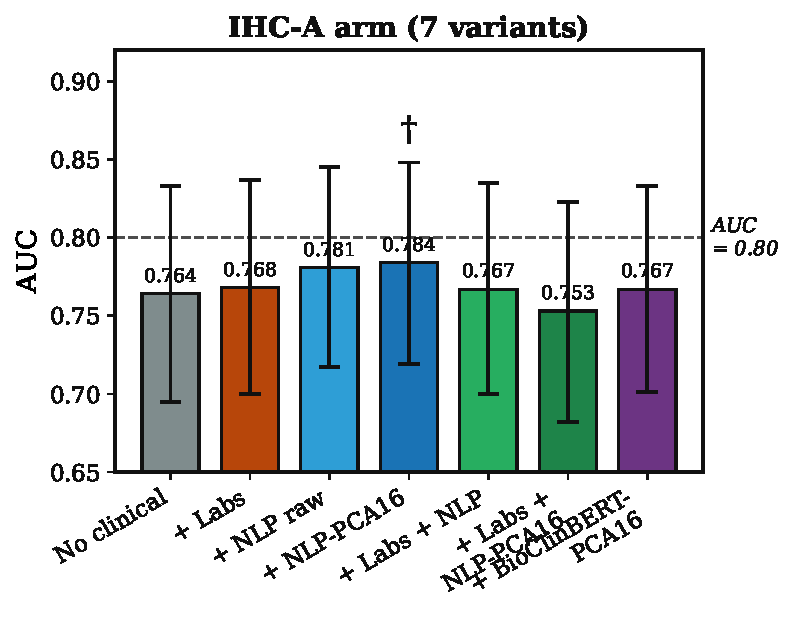
\includegraphics[width=0.48\textwidth]{figures/fig3a_auc_ihca_demo.pdf}}
  \hfill
  \subfloat[IHC-G arm (4 variants)\label{fig:auc_ihcg}]{%
    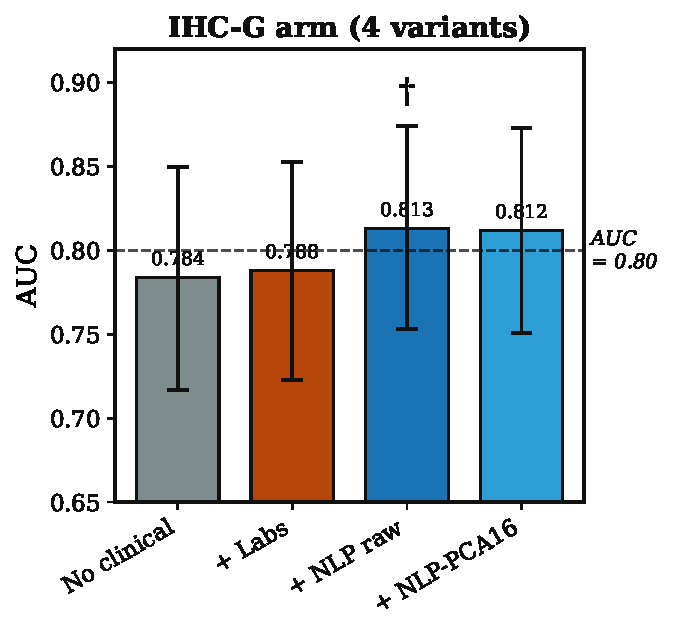
\includegraphics[width=0.48\textwidth]{figures/fig3b_auc_ihcg_demo.pdf}}
  \caption{AUC comparison across clinical encoding strategies for
    (\textbf{A}) the IHC-A arm and (\textbf{B}) the IHC-G arm. Bars show
    pooled out-of-fold AUC from 10-fold cross-validation ($n = 247$); error
    bars denote DeLong 95\% confidence intervals. The dashed horizontal line
    at AUC~$=0.80$ indicates the conventional threshold for clinically
    useful discrimination. $^\dagger$Best-performing model overall (DyAM
    Rad+IHC-G+Gen+PDL1+NLP raw, AUC~$=0.813$).}
  \label{fig:auc_comparison}
\end{figure}

%% ═══════════════════════════════════════════════════════════════════════════
%% B9 — Survival Analysis
%% ═══════════════════════════════════════════════════════════════════════════

\subsection{Survival Analysis: NLP Encoding Enhances Independent Prognostic Value}
\label{sec:survival}

The DyAM risk score was a statistically significant independent prognostic
factor for PFS across all eight model variants in multivariate Cox regression
(all $p < 0.001$, adjusted for age, ECOG performance status, serum albumin,
dNLR, and liver metastasis status; Table~\ref{tab:survival}).

\paragraph{Cox hazard ratios.}
NLP-PCA16 yielded the highest hazard ratio in the IHC-A arm
(HR~$= 6.07$, 95\%~CI: 3.50--10.52), compared with HR~$= 5.30$
[3.10--9.07] for the no-clinical baseline and HR~$= 5.31$ [2.88--9.79]
for numeric labs.
In the IHC-G arm, NLP raw achieved HR~$= 4.97$ [2.98--8.31] versus
HR~$= 4.74$ [2.82--7.97] for no-clinical and
HR~$= 4.49$ [2.56--7.89] for numeric labs.
Notably, numeric labs did not improve the hazard ratio in either arm,
whereas NLP encoding consistently increased it, suggesting that
sentence-embedded clinical context captures prognostic information
not represented by the five Cox covariates or by raw numeric features.

\paragraph{Time-dependent AUC.}
The advantage of NLP encoding was time-dependent:
in the IHC-A arm, NLP-PCA16 improved time-dependent AUC
by $+0.024$ at 12~months and $+0.020$ at 18~months relative to the
no-clinical baseline, with smaller differences at 6~months ($+0.002$).
This pattern, concentrated at late timepoints, is consistent with the
hypothesis that sentence embeddings primarily encode long-term
survival characteristics rather than short-term binary response.

\paragraph{C-index.}
Harrell's C-index showed a consistent but modest improvement with
NLP variants ($\Delta C = +0.005$ in both IHC arms;
Wilcoxon $p = 0.492$ and $p = 0.375$ for IHC-A and IHC-G, respectively),
which did not reach statistical significance.
The high inter-fold variance (range 0.52--0.78 across 10 folds)
and the small fold size ($\approx$25 patients per fold) explain the
non-significant result independently of the true effect size.

\paragraph{Calibration.}
All models were well-calibrated, with Integrated Brier Scores of
0.172--0.175, well below the 0.25 random-classifier baseline.
NLP-PCA16 in the IHC-A arm achieved the lowest IBS (0.1716),
indicating marginally superior probabilistic calibration.

\paragraph{Kaplan--Meier stratification.}
Dichotomising patients at risk score~$=0$ produced statistically significant
separation between high- and low-risk groups for all eight models
($p < 0.005$ by log-rank test; Table~\ref{tab:km}), with the highest
$\chi^2$ statistic observed for the IHC-G arm with NLP raw clinical encoding
($\chi^2 = 28.92$). Representative curves are shown in
Figure~\ref{fig:km_curves}, and a summary of all survival metrics is shown
in Figure~\ref{fig:survival_summary}.

%% tables/table4_survival.tex
\begin{table}[H]
\caption{Survival analysis results across all model variants.
  Discovery cohort ($n = 247$; 209 events, 84.6\%; median PFS 2.7~months).
  C-index: Harrell's concordance index with bootstrap 95\%~CI (1{,}000
  resamples). Cox HR: hazard ratio from multivariate Cox proportional
  hazards regression adjusted for age, ECOG, albumin, dNLR, and liver
  metastases (95\%~CI; Wald $p$-value). tdAUC: time-dependent AUC at
  12~months. IBS: Integrated Brier Score (lower is better;
  $< 0.25$ indicates better-than-random calibration).
  All Cox $p < 0.001$.
  Bold: best value per column within each IHC arm.}
\label{tab:survival}
\small
\begin{tabular}{@{}p{3.4cm}ccccc@{}}
\toprule
\textbf{Model} &
\textbf{C-index} & \textbf{[95\%~CI]} &
\textbf{Cox HR} & \textbf{[95\%~CI]} &
\textbf{IBS} \\
\midrule
\multicolumn{6}{l}{\textit{IHC-A arm}} \\
No clinical          & 0.623 & [0.580--0.665] & 5.30 & [3.10--9.07]   & 0.1745 \\
+ Labs               & 0.626 & [0.583--0.669] & 5.31 & [2.88--9.79]   & 0.1739 \\
+ NLP raw            & 0.625 & [0.583--0.663] & 5.91 & [3.40--10.25]  & 0.1723 \\
\textbf{+ NLP-PCA16} & \textbf{0.628} & \textbf{[0.584--0.668]}
                     & \textbf{6.07} & \textbf{[3.50--10.52]}
                     & \textbf{0.1716} \\
\midrule
\multicolumn{6}{l}{\textit{IHC-G arm}} \\
No clinical          & 0.626 & [0.583--0.665] & 4.74 & [2.82--7.97]  & 0.1748 \\
+ Labs               & \textbf{0.632} & \textbf{[0.587--0.675]} & 4.49 & [2.56--7.89]  & 0.1746 \\
\textbf{+ NLP raw}   & \textbf{0.632} & \textbf{[0.591--0.672]}
                     & \textbf{4.97} & \textbf{[2.98--8.31]}
                     & \textbf{0.1736} \\
+ NLP-PCA16          & 0.631 & [0.590--0.672] & 4.69 & [2.86--7.68]  & 0.1736 \\
\bottomrule
\end{tabular}
\end{table}

%% tables/table5_km.tex
\begin{table}[H]
\caption{Kaplan--Meier log-rank statistics for survival stratification.
  Patients were dichotomised at risk score~$= 0$.
  Threshold for significance: $\chi^2 > 7.88$ ($p < 0.005$).
  All models achieve $p < 0.005$.
  $\star$ Highest $\chi^2$ across all tested models.}
\label{tab:km}
\begin{tabular}{llcc}
\toprule
\textbf{Model} & \textbf{IHC arm} & \boldmath{$\chi^2$} & \textbf{$p$-value} \\
\midrule
DyAM No clinical & IHC-A & 28.17 & $< 0.005$ \\
DyAM + NLP-PCA16 & IHC-A & 23.74 & $< 0.005$ \\
DyAM No clinical & IHC-G & 20.07 & $< 0.005$ \\
\textbf{DyAM + NLP-PCA16} & \textbf{IHC-G} & \textbf{28.92}$^{\star}$ & $\mathbf{< 0.005}$ \\
\bottomrule
\end{tabular}
\end{table}


\begin{figure}[H]
  \centering
  \subfloat[IHC-A, no clinical ($\chi^2 = 28.17$)]{%
    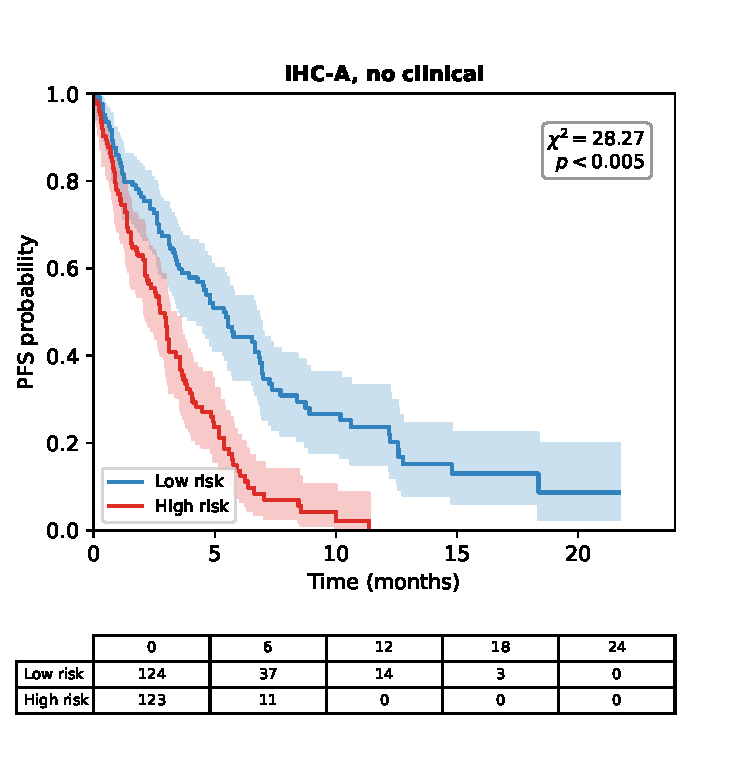
\includegraphics[width=0.48\textwidth]{figures/fig4a_km_ihca_noclin.pdf}}
  \hfill
  \subfloat[IHC-A, + NLP-PCA16 ($\chi^2 = 23.74$)]{%
    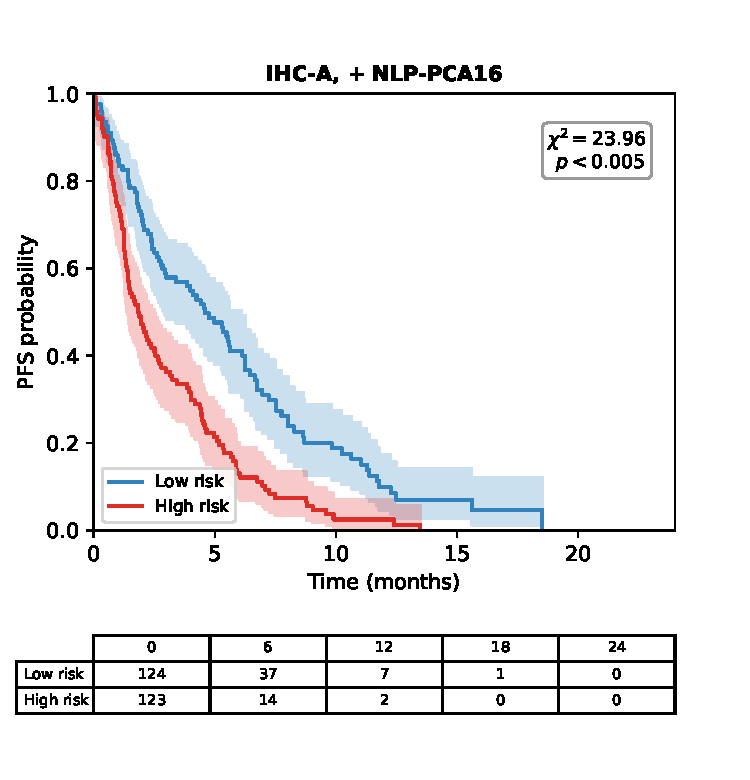
\includegraphics[width=0.48\textwidth]{figures/fig4b_km_ihca_nlppca16.pdf}}

  \subfloat[IHC-G, no clinical ($\chi^2 = 20.07$)]{%
    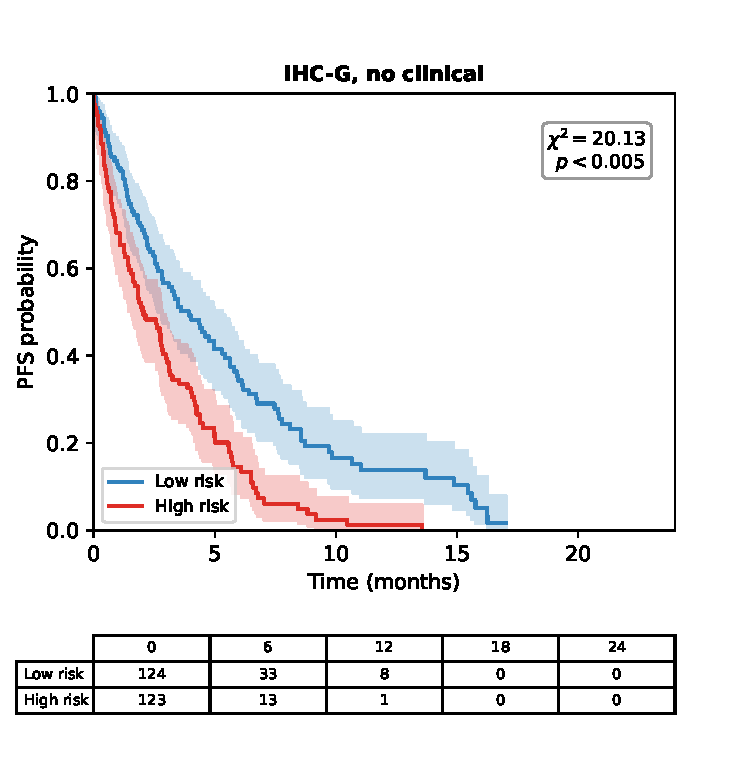
\includegraphics[width=0.48\textwidth]{figures/fig4c_km_ihcg_noclin.pdf}}
  \hfill
  \subfloat[IHC-G, + NLP raw ($\chi^2 = 28.92^{\star}$)]{%
    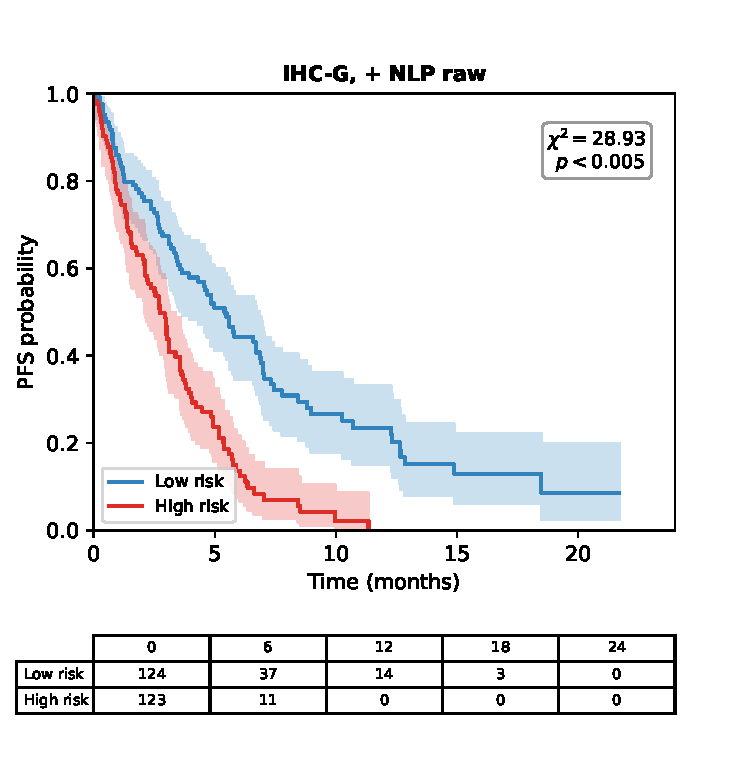
\includegraphics[width=0.48\textwidth]{figures/fig4d_km_ihcg_nlpraw.pdf}}
  \caption{Kaplan--Meier progression-free survival curves for representative
    models, stratified at risk score~$=0$ into high-risk (red) and low-risk
    (blue) groups, with number-at-risk tables.
    (\textbf{A}) IHC-A arm, no clinical encoding.
    (\textbf{B}) IHC-A arm with NLP-PCA16 clinical encoding.
    (\textbf{C}) IHC-G arm, no clinical encoding.
    (\textbf{D}) IHC-G arm with NLP raw clinical encoding
    ($^{\star}$the highest log-rank statistic among all tested models).
    All comparisons reach $p < 0.005$ by the log-rank test.}
  \label{fig:km_curves}
\end{figure}

\begin{figure}[H]
  \centering
  \subfloat[Harrell's C-index (bootstrap 95\% CI)]{%
    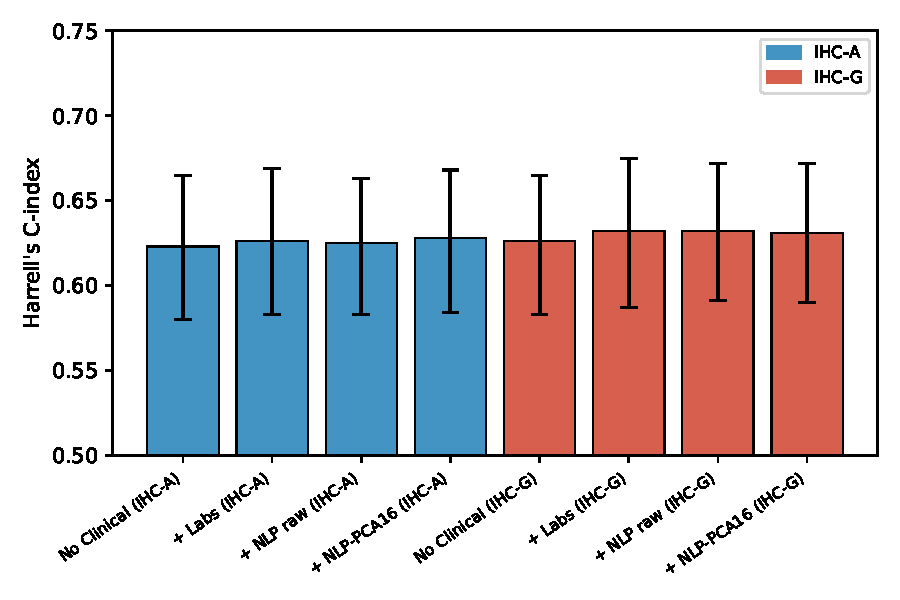
\includegraphics[width=0.48\textwidth]{figures/fig5a_cindex.pdf}}
  \hfill
  \subfloat[Time-dependent AUC (6/12/18~months)]{%
    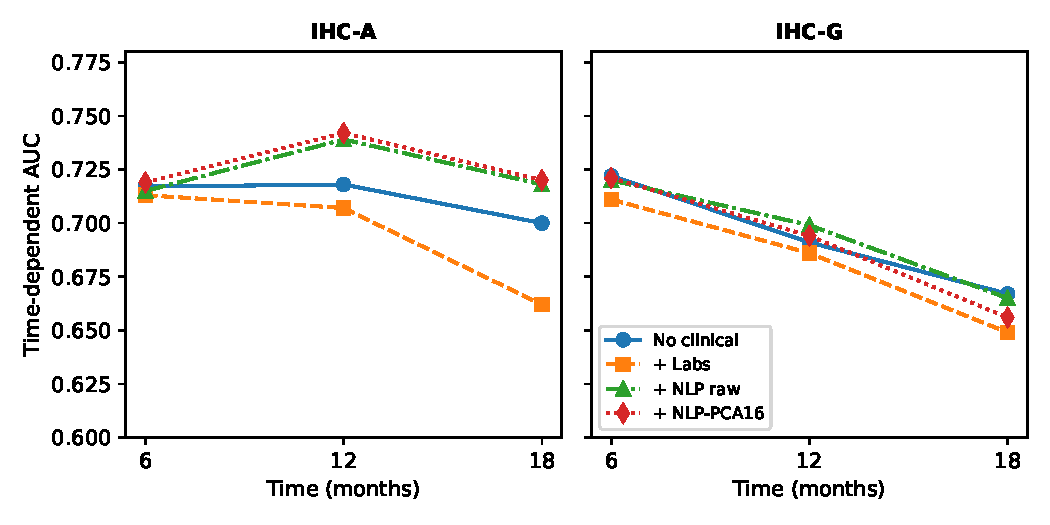
\includegraphics[width=0.48\textwidth]{figures/fig5b_tdauc.pdf}}

  \subfloat[Multivariate Cox hazard ratios (forest plot)]{%
    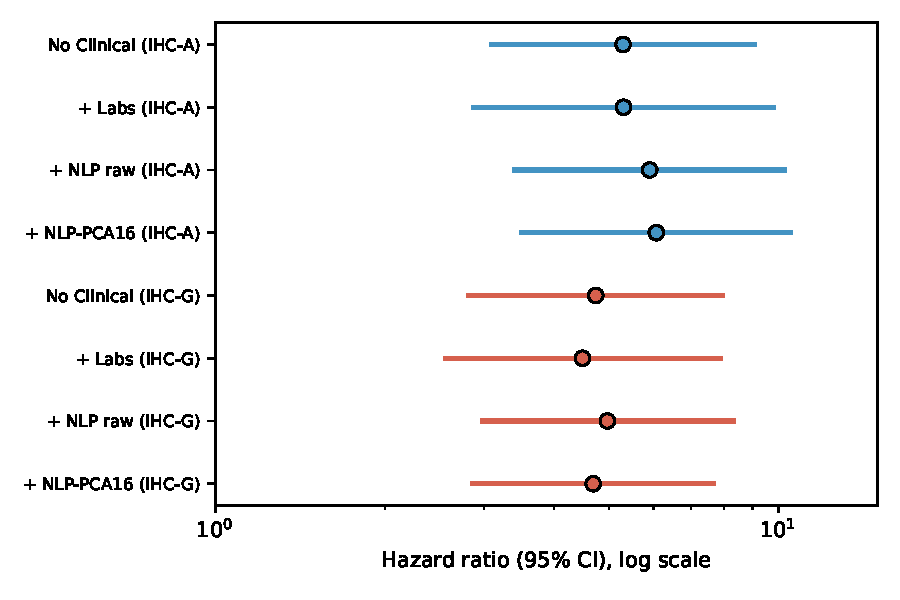
\includegraphics[width=0.48\textwidth]{figures/fig5c_cox_forest.pdf}}
  \hfill
  \subfloat[Integrated Brier Score]{%
    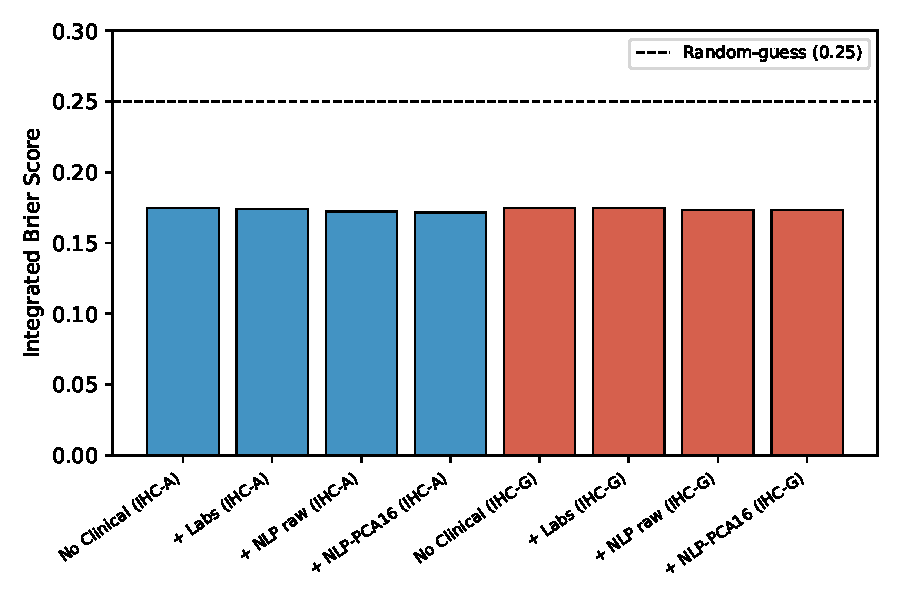
\includegraphics[width=0.48\textwidth]{figures/fig5d_ibs.pdf}}
  \caption{Survival analysis summary across clinical encoding strategies.
    (\textbf{A}) Harrell's C-index with bootstrap 95\% confidence intervals
    for IHC-A and IHC-G arms; differences between encoding strategies were
    not statistically significant (paired Wilcoxon $p > 0.05$).
    (\textbf{B}) Time-dependent AUC at 6, 12, and 18~months; NLP-encoded
    models show the largest advantage at 12--18~months.
    (\textbf{C}) Forest plot of multivariate Cox proportional hazards ratios
    for the fused risk score, adjusted for age, ECOG performance status,
    albumin, derived neutrophil-to-lymphocyte ratio, and liver metastases
    (all $p < 0.001$).
    (\textbf{D}) Integrated Brier Score (IBS) for each model; all values
    fall well below the 0.25 random-guess threshold (range
    0.172--0.175), indicating good calibration across all encoding
    strategies.}
  \label{fig:survival_summary}
\end{figure}
